\documentclass[t,12pt]{beamer}
\definecolor{links}{RGB}{0, 104, 172}
\definecolor{red}{rgb}{0.702,0.106,0.106} 
\hypersetup{colorlinks=true,urlcolor=links}
\usetheme{default}
% we need to change to Cornell red
\definecolor{beamer@blendedblue}{rgb}{0.702,0.106,0.106} 
\beamertemplatenavigationsymbolsempty
\setbeamerfont{institute}{size={\fontsize{10}{10}}}

\usepackage[english]{babel}
\usepackage{fontspec}
\setsansfont{TeX Gyre Heros}

\title{HD4630 Workshops}
\subtitle{A practical introduction to fMRI Analysis}
\author{Elizabeth DuPre \\[.8\baselineskip]}

\vspace{2ex}
\institute{Human Neuroscience Institute 
\\[4pt]
\href{http://www.human.cornell.edu/hd/}{Department of Human Development}
\\[4pt]
\href{https://www.cornell.edu/}{Cornell University}}
\date{}

\begin{document}

\begin{frame}
  \titlepage
\end{frame}

\section{Introduction}
% First Slide
\begin{frame}{Why Workshops?}
\vspace{4pt}
\begin{itemize}
\setlength\itemsep{0.75em}
  \item You'll spend a lot of time this semester \\
  learning what fMRI \textit{is}
  \item I'm here to help you figure out how to \textit{do} it
  \item We'll be using the software package \href{https://afni.nimh.nih.gov/afni/}{AFNI} \\
  \vspace{4pt}
  \begin{tabular}{c l}
	 \textbf{A} & nalysis of  \\
	 \textbf{F} & unctional   \\
     \textbf{N} & euro        \\
     \textbf{I} & maging Data \\
  \end{tabular}
\end{itemize}
\begin{figure}
\raggedleft
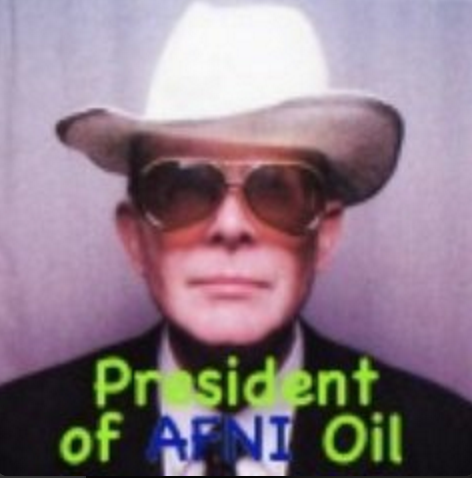
\includegraphics[width=.275\textwidth]{images/AFNIman.png}
\end{figure}
\end{frame}

% Second Slide
\begin{frame}{AFNI for All!}
\vspace{10pt}
\begin{itemize}
\setlength\itemsep{1em}
  \item AFNI is designed to work in posix environments
  \vspace{4pt}
  \begin{itemize}
   \item So it won't work on your Windows computer
  \end{itemize}
  \item We want AFNI for everyone, so we'll be using software containerization
  \vspace{4pt}
  \begin{itemize}
   \item Specifically with \href{https://www.docker.com/products/docker}{Docker} or \href{https://www.docker.com/products/docker-toolbox}{Docker Toolbox} 
  \end{itemize}
\end{itemize}
\begin{figure}
\centering

\includegraphics[width=.4\textwidth]{images/docker_whale.png}
\end{figure}
\end{frame}

% Third Slide
\begin{frame}{What's with the whale?}
\begin{figure}
\centering
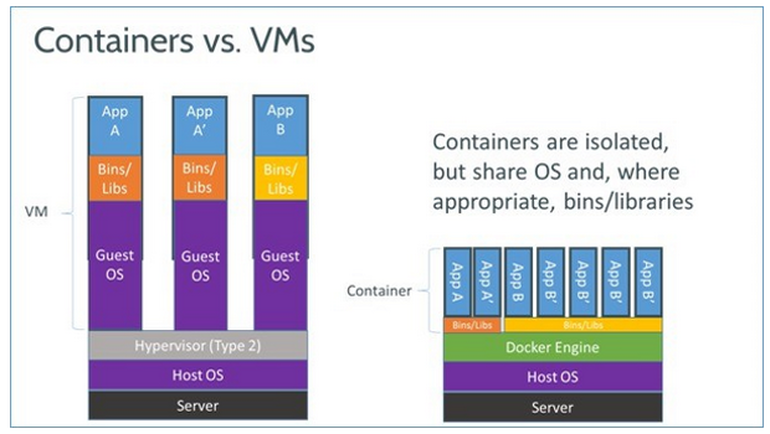
\includegraphics[width=\textwidth]{images/docker_vs_vm.png}
\end{figure}
\begin{block}{Learning More}
A great tutorial on containerization is available \href{https://www.digitalocean.com/community/tutorials/the-docker-ecosystem-an-overview-of-containerization}{here}
\end{block}
\end{frame}

% Fourth Slide
\begin{frame}{You Can Haz Data}
\vspace{10pt}
\begin{itemize}
\setlength\itemsep{1em}
  \item One practical element we won't cover is data collection
  \item Instead, we'll be using publicly available task data from \href{https://openfmri.org/}{OpenfMRI}
  \vspace{4pt}
  \begin{itemize}
  \setlength\itemsep{0.5em}
    \item A \href{https://openfmri.org/dataset/ds000102/}{Flanker task} collected at NYU
    \item A \href{https://openfmri.org/dataset/ds000164/}{Stroop task} collected at Carnegie Mellon
  \end{itemize}
\end{itemize}
\end{frame}

\section{Getting Started}

% Fifth Slide
\begin{frame}{Our Plan Today}
\vspace{10pt}
\begin{itemize}
\setlength\itemsep{1em}
  \item We need to install Docker or Docker Toolbox, along with a few additional dependencies
  \vspace{4pt}
  \begin{itemize}
  \setlength\itemsep{0.5em}
    \item A virtualization client
    \item An \href{https://en.wikipedia.org/wiki/X_Window_System}{X11 server}
  \end{itemize}
  \item The exact make and model of these dependencies will vary by your operating system (OS)
    \item A complete guide for installing Docker on each OS will be made available for you
\end{itemize}
\end{frame}

% Sixth Slide
\begin{frame}{What Next?}
\vspace{10pt}
\begin{itemize}
\setlength\itemsep{1em}
  \item The most important command today will be \\
  \vspace{2pt}
  \texttt{docker pull emdupre/hd4630\char`_workshops}
  \vspace{4pt}
  \begin{itemize}
  \setlength\itemsep{0.5em}
    \item We need to 'pull' our Docker image containing \\
    all the relevant software
  \end{itemize}
  \item You'll also need to download the data from \\
  OpenfMRI
  \vspace{4pt}
  \begin{itemize}
  \setlength\itemsep{0.5em}
    \item This can be done any time before our next full workshop
  \end{itemize}
\end{itemize}
\end{frame}

% Seventh Slide
\begin{frame}[plain,c]
\begin{center}
{\color{red} \LARGE Let's get started!}
\end{center}
\end{frame}

\end{document}
